\documentclass[12pt]{article}
\linespread{1.25}
\usepackage{times}

\usepackage{pgfplots}
\pgfplotsset{compat = newest}
\usetikzlibrary{positioning, arrows.meta}
\usepgfplotslibrary{fillbetween}
\usepackage{amsmath}
\begin{document}
          \begin{center}
               \hspace*{-4cm}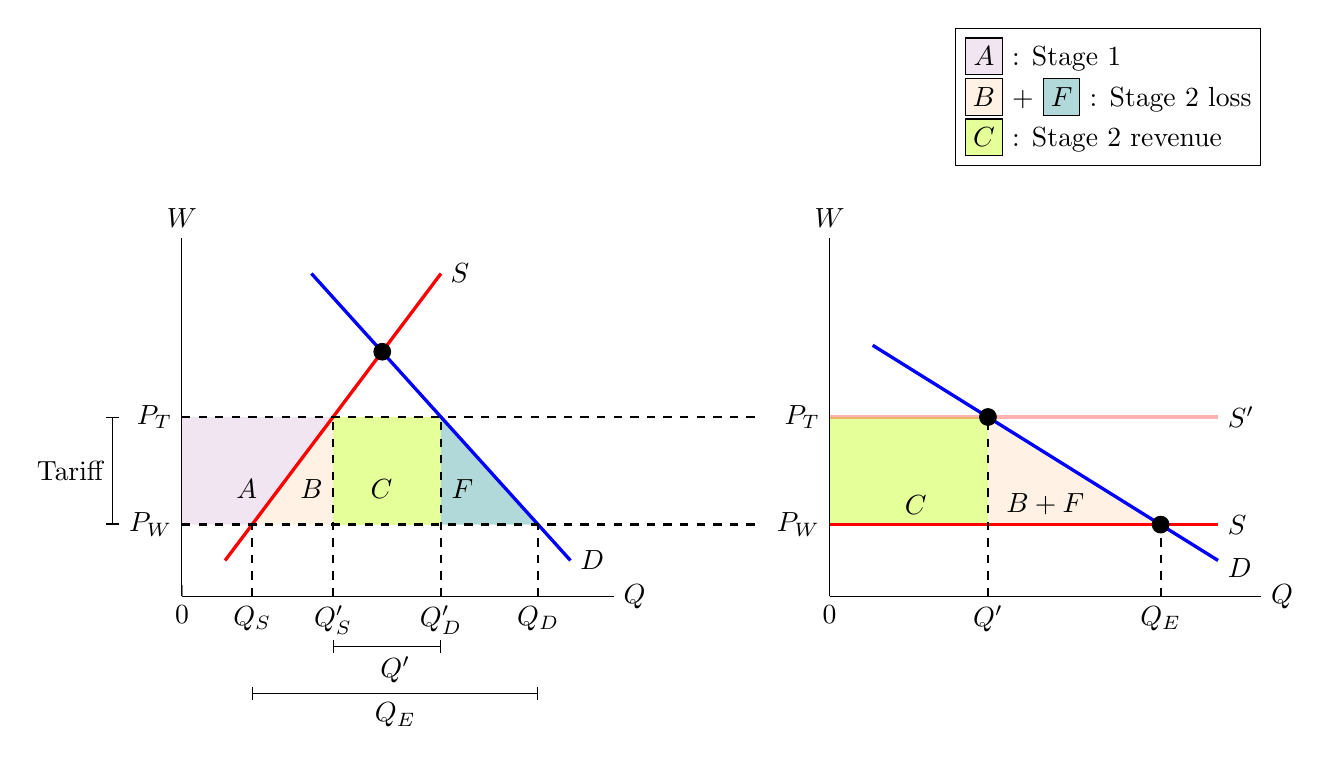
\begin{tikzpicture}
                                 % Domestic market
                                     \begin{axis}[
                                                  scale = 0.8,
                                                  xmin = 0, xmax = 10,
                                                  ymin = 0, ymax = 10,
                                                  axis lines* = left,
                                                  xtick = {0}, ytick = \empty,
                                                  axis on top,
                                                  clip = false,
]

% Colouring areas
                 \fill[violet, opacity = 0.1] (0, 2) -- (1.63, 2) -- (3.5, 5) -- (0, 5);
                 \fill[orange, opacity = 0.1] (1.63, 2) -- (3.5, 2) -- (3.5, 5);
                 \fill[teal, opacity = 0.3] (6, 2) -- (8.25, 2) -- (6, 5);
                 \fill[lime, opacity = 0.4] (3.5, 2) -- (6, 2) -- (6, 5) -- (3.5, 5);


% Supply and demand curves
                 \addplot[color = red, very thick] coordinates{(1, 1) (6, 9)};
                 \addplot[color = blue, very thick] coordinates {(3, 9) (9, 1)};


% Dashed lines
                 \addplot[color = black, dashed, thick] coordinates {(0, 2) (13.4, 2)};
                 \addplot[color = black, dashed, thick] coordinates {(0, 5) (13.4, 5)};
                 \addplot[color = black, dashed, thick] coordinates {(1.63, 0) (1.63, 2)};
                 \addplot[color = black, dashed, thick] coordinates {(3.5, 0) (3.5, 5)};
                 \addplot[color = black, dashed, thick] coordinates {(6, 0) (6, 5)};
                 \addplot[color = black, dashed, thick] coordinates {(8.25, 0) (8.25, 2)};


% Coordinate points
                 \addplot[color=black, mark=*, only marks, mark size=3pt] coordinates {(4.64, 6.82)};



% Labels
                 \node [above] at (current axis.above origin) {$W$};
                 \node [right] at (current axis.right of origin) {$Q$};
                 \node [right] at (6, 9) {$S$};
                 \node [right] at (9, 1) {$D$};
                 \node [below] at (1.63, 0) {$Q_S$};
                 \node [below] at (3.5, 0) {$Q_S^\prime$};
                 \node [below] at (6, 0) {$Q_D^\prime$};
                 \node [below] at (8.25, 0) {$Q_D$};
                 \node [left] at (0, 2) {$P_W$};
                 \node [left] at (0, 5) {$P_T$};
                 \node at (1.5, 3) {$A$};
                 \node at (3, 3) {$B$};
                 \node [left] at (5.1, 3) {$C$};
                 \node at (6.5, 3) {$F$};



% Dimension lines
                 \draw[|-|] (3.5, -1.4) to (6, -1.4);
                 \node [below] at (4.94, -1.4) {$Q^\prime$};
                 \draw[|-|] (1.63, -2.7) to (8.25, -2.7);
                 \node [below] at (4.94, -2.7) {$Q_E$};
                 \draw[|-|] (-1.6, 2) to (-1.6, 5);
                 \node [left] at (-1.6, 3.5) {Tariff};
         \end{axis}


% Import market
                \begin{axis}[
                             scale = 0.8,
                             xmin = 0, xmax = 10,
                             ymin = 0, ymax = 10,
                             axis lines* = left,
                             xtick = {0}, ytick = \empty,
                             axis on top,
                             clip = false,
                             shift = {(axis cs: 15, 0)},
]

% Colouring areas
                 \fill[lime, opacity = 0.4] (0, 2) -- (3.67, 2) -- (3.67, 5) -- (0, 5);
                 \fill[orange, opacity = 0.1] (3.67, 2) -- (3.67, 5) -- (7.67, 2);


% Supply and demand curves
                \addplot[color = red, very thick] coordinates{(0, 2) (9, 2)};
                \addplot[color = red, opacity = 0.3, very thick] coordinates{(0, 5) (9, 5)};
                \addplot[color = blue, very thick] coordinates {(1, 7) (9, 1)};


% Dashed lines
                \addplot[color = black, dashed, thick] coordinates {(3.67, 0) (3.67, 5)};
                \addplot[color = black, dashed, thick] coordinates {(7.67, 0) (7.67, 2)};


% Coordinate points
                \addplot[color=black, mark=*, only marks, mark size=3pt] coordinates {(3.67, 5) (7.67, 2)};


% Labels
                 \node [above] at (current axis.above origin) {$W$};
                 \node [right] at (current axis.right of origin) {$Q$};
                 \node [right] at (9, 2) {$S$};
                 \node [right] at (9, 5) {$S^\prime$};
                 \node [right] at (9, 0.8) {$D$};
                 \node [below] at (3.67, 0) {$Q^\prime$};
                 \node [below] at (7.67, 0) {$Q_E$};
                 \node [left] at (0, 2) {$P_W$};
                 \node [left] at (0, 5) {$P_T$};
                 \node [above] at (2, 2) {$C$};
                 \node [above] at (5, 2) {$B + F$};


% Legend
                 \node[above left, draw, align = left] at (10, 12) {
                 \fcolorbox{black}{violet!10}{\makebox[\fontcharht\font`X]{$A$}} : Stage 1 \\
                 \fcolorbox{black}{orange!10}{\makebox[\fontcharht\font`X]{$B$}} + \fcolorbox{black}{teal!30}{\makebox[\fontcharht\font`X]{$F$}} : Stage 2 loss \\
                 \fcolorbox{black}{lime!40}{\makebox[\fontcharht\font`X]{$C$}} : Stage 2 revenue
};
                \end{axis}
          \end{tikzpicture}\hspace*{-4cm}
       \end{center}
                   \textbf{Figure 19} 

\end{document}